%%%%%%%%%%%%%%%%%%%%%%%%%%%%%%%%%%%%%%%%%%%%%%%%%%%
%
%  New template code for TAMU Theses and Dissertations starting Fall 2012.  
%  For more info about this template or the 
%  TAMU LaTeX User's Group, see http://www.howdy.me/.
%
%  Author: Wendy Lynn Turner 
%	 Version 1.0 
%  Last updated 8/5/2012
%
%%%%%%%%%%%%%%%%%%%%%%%%%%%%%%%%%%%%%%%%%%%%%%%%%%%

%%%%%%%%%%%%%%%%%%%%%%%%%%%%%%%%%%%%%%%%%%%%%%%%%%%%%%%%%%%%%%%%%%%%%%%
%%%                           SECTION II
%%%%%%%%%%%%%%%%%%%%%%%%%%%%%%%%%%%%%%%%%%%%%%%%%%%%%%%%%%%%%%%%%%%%%%

\chapter{\uppercase {Productivity \& Performance Analysis}}
The main goals of SAC are productivity and performance, but how to measure them? Programming productivity \cite{ProgramProductWiki} refers to software development issues and methodologies affecting the quantity and quality of code produced by an individual or team. The principal factors that affect productivity include learning curve (how friendly of user interface and compatibility with existing software), speed of code generation (how many lines of codes need to write) and approach to testing and maintenance (the running time at which user need to wait and debug methods). For performance issue, the execution times and job scheduling policy play key roles. The performance of a system also involves one or more characteristics such as response time, throughput, utilization of computing resources, availability or bandwidth etc. In this thesis, the (Lines of Codes) LOCs to accomplish same task and friendly user interface are discussed for measuring productivity, while execution time (speedup to sequential codes) and throughput are used for measuring performance.  

\section{Productivity Analysis}
The computer had developed from single core to multicores, but most programmers did not catch up with this trends on time. Our thinking is custom to single thread and single process applications, especially for other domain experts who did not major in computer science. For most application developers, the main tasks of programming models are trying to hide the sophisticated details and making them easy to use. To shorten the learning curve, SAC provide friendly web interface in which user only need to select and coding with template, and all other details such as data distribution, task parallelization and scheduling are transparent to user. In the view of end user, only code snippet of core algorithm need to compose, so it is even simpler than writing sequential codes. To improve usability, Breeze also provides similar operators to those in Matlab and Numpy as show in Table \ref{tab:BreezeOperators}, and all of those could be used directly in template codes of SAC. In List \ref{SeqCodeFFT}, \ref{MPICodeFFT} and \ref{SACCodeFFT}, they give a rough comparison of LOCs FFT on subvolume in sequential codes, parallel codes with MPI and template codes with SAC. Since the outlines of most seismic applications are similar, we could divide them into serval categories and abstract commonly used templates. With templates, the outline codes could be reused by all programs in same category, thus make them easy to maintain.   


%A table example is going to follow.
\begin{table}[h]
\centering
\caption{Operators in Breeze, MATLAB and Numpy}
\begin{tabular}{||l|l|l|l||}
\hline
Elementwise addition & a + b & a + b & a + b \\
\hline
Elementwise multiplication & a :* b & a .* b & a * b \\
\hline
Elementwise comparison & a :\textless{}  b & a \textless{}  b & a \textless{}  b \\
\hline
Inplace addition & a :+= 1.0 & a += 1 & a += 1 \\
\hline
Inplace elementwise multiplication & a :*= 2.0 & a *= 2 & a *= 2 \\
\hline
Vector dot product & a dot b & dot(a,b)	& dot(a,b) \\
\hline
Elementwise sum	& sum(a) & sum(sum(a)) & a.sum() \\
\hline
Elementwise max & a.max & max(a) & a.max() \\
\hline
Elementwise argmax & argmax(a) & argmax(a) & a.argmax() \\
\hline
Ceiling	& ceil(a) & ceil(a) & ceil(a) \\
\hline
Floor	& floor(a) & floor(a) & floor(a) \\
\hline
\end{tabular}
\label{tab:BreezeOperators}
\end{table}
%%%%%%%%%%%%%%%%%%%%%%%%%%%%%%%%%%%%%%%%%%%%%%%%%%%%%%

\lstset{language=Java,frame=single}
\begin{lstlisting}[float,caption= Sequential Pseudo Codes of FFT on Subvolume, label=SeqCodeFFT]
//Sequential codes
int applyFFTOnSubvolume() 
{
   while(remain splits > 0) 
   {
      for(i <- 0 until iSplit)
      {
         for(j <- 0 until jDim)
         {
            for(k <- 0 until kDim)
            {
               subVol <- get all neighbour pixels in 3 loops
               val dv = new DenseVector(subVol);
               val fftres = fourierTr(dv).map(a=>a.abs.toFloat); 
               res(i*kDim*jDim+j*kDim+k) = max(fftres);
            }
         }
      }
      get next split;
   }
}
\end{lstlisting}

\lstset{language=Java,frame=single}
\begin{lstlisting}[float,caption= Pseudo Codes of FFT on Subvolume in MPI, label=MPICodeFFT]
//MPI Codes
int computeFFTOnSubvolume() 
{
   while(remain splits > 0) 
   {    
      divide split into small chunk
      scatter chunks to all worker processes
      for(i <- 0 until iSplit)
      {
         for(j <- 0 until jDim)
         {
            for(k <- 0 until kDim)
            {
               subVol <- get all neighbour pixels in 3 loops
               val dv = subVol to vector;
               val fftres = doFFT on dv; 
               res(i*kDim*jDim+j*kDim+k) = max(fftres);
            }
         }
      }
      gather chunks from all worker processes 
      get next split;
   }
}
\end{lstlisting}

\lstset{language=Java,frame=single}
\begin{lstlisting}[float,caption= Sample Codes of FFT on Subvolume in Template of SAC,label=SACCodeFFT]
//Sample Template Codes in SAC
class PixelApplication extends java.io.Serializable {
     def processPixel(volume:Array[Float]):Float = {
         val dv = new DenseVector(volume);
         val fftres = fourierTr(dv).map(a=>a.abs.toFloat); 
         max(fftres)
     }
}
\end{lstlisting}


\section{Performance Analysis}
There are a lot of tools used for measuring performance of application. To get the execution time, wall clock is the simplest way. But if we want to make some deep analysis to find the bottleneck, more information such as CPU usage, memory usage, disk I/O and network communication metrics need to be collected. The situation becomes more complex if application run in multithread or run on multi-nodes with synchronization. Spark itself provide web UI for monitoring of resource usage of whole cluster, task running status and detail of each stage in task. Nigel's performance Monitor (nmon) could collect miscellaneous metrics information on each node, and Nmon Analyzer could visualize such information for deep analysis. So we use wall clock to get total running time and execution of each stage for sequential codes, and use Spark web monitor UI to get execution time of parallel codes running on Spark. Each node will launch nmon to collect runtime information at the same time of application starts, and then all of these data are merged together, feed to Nmon Analyzer for deep study. 

Due to the speed gap between CPU and I/O device such as network or hard disk, main memory has always been the most valuable resource in computer system. Spark boosts computing performance by caching  RDD in memory, but it also bring problem of competition for memory. Without careful plan on memory usage, it will even hold up the overall performance. Spark is running on JVM, so we turn on the GC log option while launching a job, and also use Nmon to monitor memory usage. Basing on running results, we will first get abnormal cases, and then in such case, CPU, Memory, Network I/O and Disk I/O will be inspected in sequence.  

\ifx true false
%%%%%%%%%%%%%%%%%%%%%%%%%%%%%%%%%%%%%%%%%%%%%%%%%%%%%%%
\begin{figure}[h]
%\centering
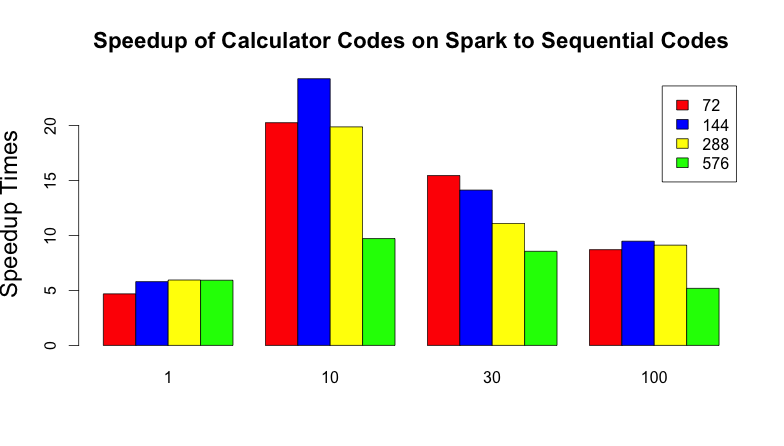
\includegraphics[scale=.60]{figures/CalcSpeedup.png}
\caption{Speedup of Calculator Codes}
\label{CalcSpeedup}
\end{figure}
%%%%%%%%%%%%%%%%%%%%%%%%%%%%%%%%%%%%%%%%%%%%%%%%%%%%%%%
\fi 


The running time information is alreay given in previous chapter, and the speedup factors for each applicaton are shown in Figure \ref{HtfSpeedup}, \ref{FFTSpeedup}, \ref{HistSpeedup} and \ref{JacobiSpeedup}. we will make analysis on them respectively in the following sections. 

\subsection{Performance Analysis of Hilbert Transformation Filter}
Figure \ref{HtfSpeedup} show the speedup information of parallel codes on Spark to sequential codes. There is a positive correlation between number of cores and performance in almost each split. The performance boost from 288 cores to 576 cores is not obvious, because 576 cores run in hyper-thread mode. The best  speedup is located at 10 lines split with 576 cores, and the performance decrease slightly after increasing split size to 30 lines or 100 lines.

%%%%%%%%%%%%%%%%%%%%%%%%%%%%%%%%%%%%%%%%%%%%%%%%%%%%%%%
\begin{figure}[h]
%\centering
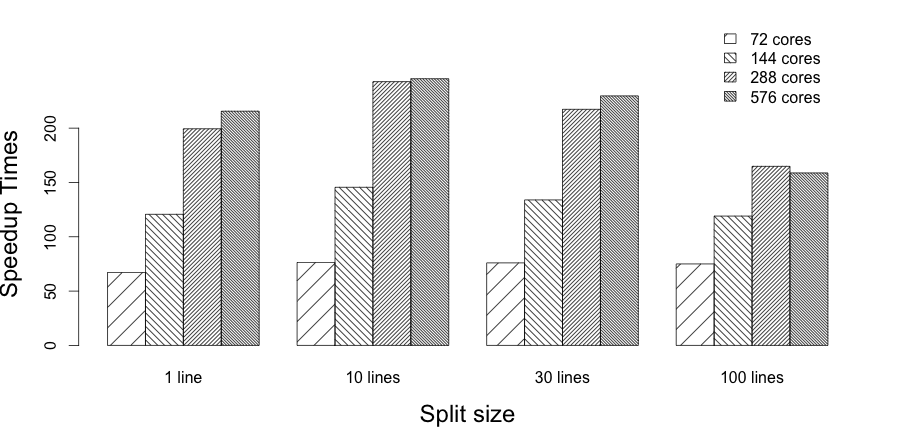
\includegraphics[scale=.50]{figures/HtfSpeedup.png}
\caption{Speedup of Hilbert Transform Filter Codes}
\label{HtfSpeedup}
\end{figure}
%%%%%%%%%%%%%%%%%%%%%%%%%%%%%%%%%%%%%%%%%%%%%%%%%%%%%%%


\begin{figure}[h]
\centering
\begin{subfigure}{1\textwidth}
  \centering
  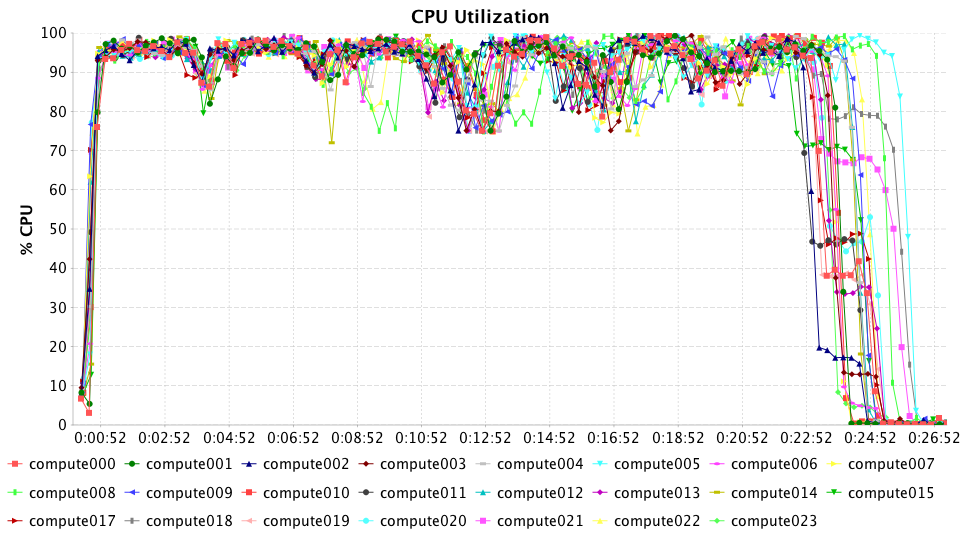
\includegraphics[width=1\linewidth]{figures/Htf10_576_CPU.png}
  \caption{CPU Usage}
  \label{Htf10_576_CPU}
\end{subfigure}
\begin{subfigure}{1\textwidth}
  \centering
  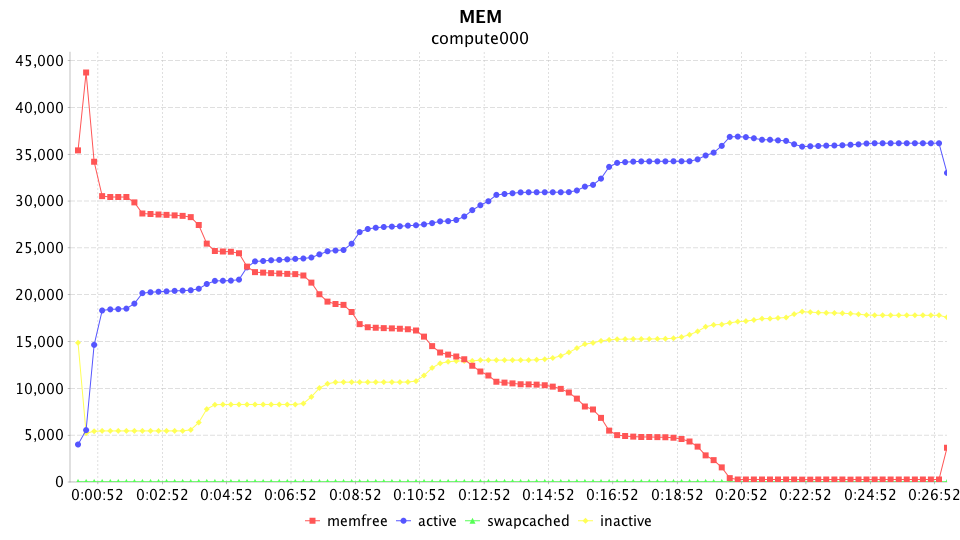
\includegraphics[width=1\linewidth]{figures/Htf10_576_MEM.png}
  \caption{Memory Usage}
  \label{Htf10_576_MEM}
\end{subfigure}
\caption{Resource Usage of Hilbert Transform Filter with 10 Lines per Split and 576 Cores}
\label{Htf10_576}
\end{figure}


\begin{figure}[h]
\centering
\begin{subfigure}{1\textwidth}
  \centering
  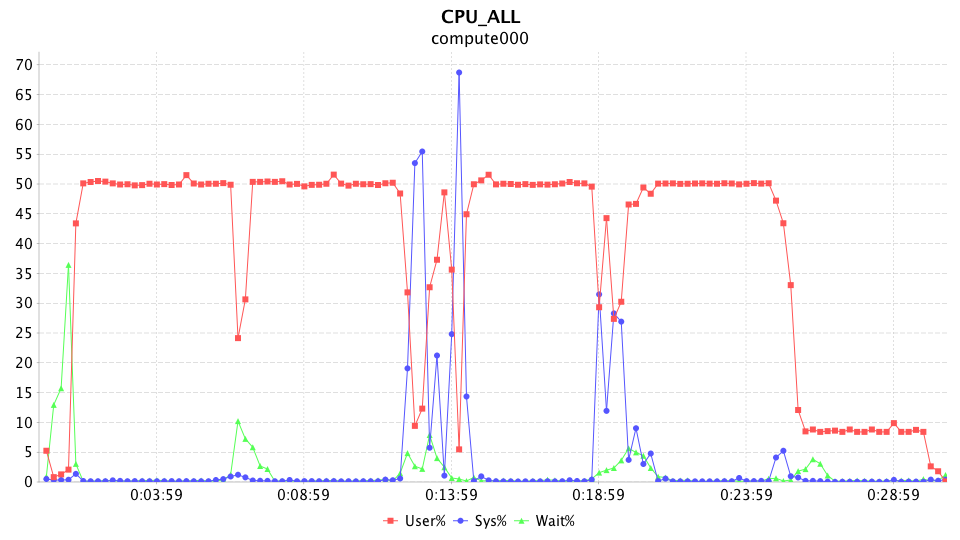
\includegraphics[width=1\linewidth]{figures/Htf30_288_CPU.png}
  \caption{CPU Usage}
  \label{Htf30_288_CPU}
\end{subfigure}
\begin{subfigure}{1\textwidth}
  \centering
  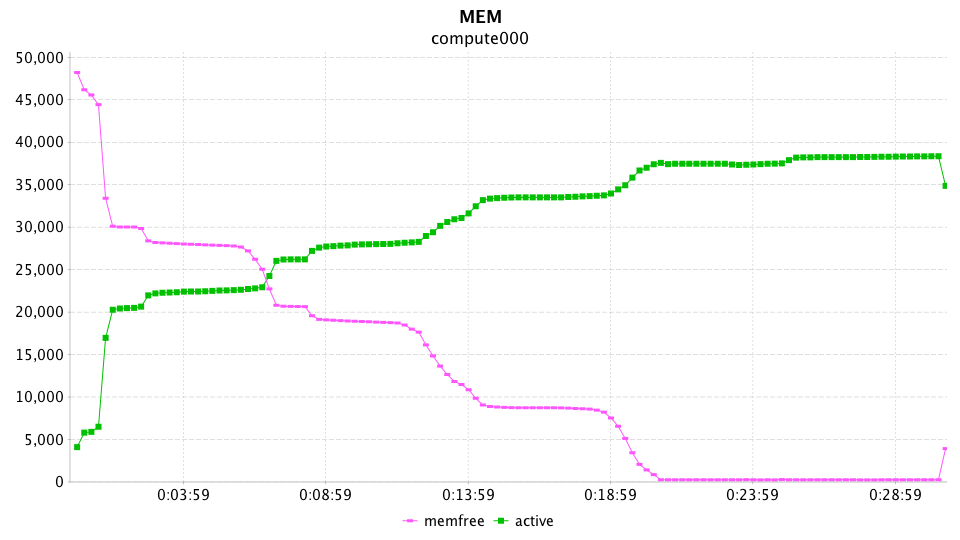
\includegraphics[width=1\linewidth]{figures/Htf30_288_MEM.png}
  \caption{Memory Usage}
  \label{Htf30_288_MEM}
\end{subfigure}
\caption{Resource Usage of Hilbert Transform Filter with 30 Lines per Split and 288 Cores}
\label{Htf30_288}
\end{figure}


\subsection{Performance Analysis of FFT}

%%%%%%%%%%%%%%%%%%%%%%%%%%%%%%%%%%%%%%%%%%%%%%%%%%%%%%%
\begin{figure}[h]
%\centering
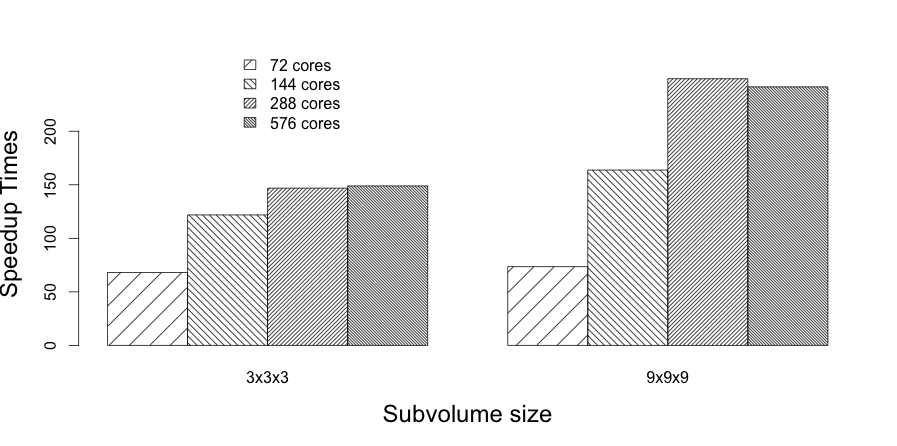
\includegraphics[scale=.50]{figures/FFTSpeedup.png}
\caption{Speedup of FFT Codes}
\label{FFTSpeedup}
\end{figure}
%%%%%%%%%%%%%%%%%%%%%%%%%%%%%%%%%%%%%%%%%%%%%%%%%%%%%%%
 

\begin{figure}[h]
\centering
\begin{subfigure}{1\textwidth}
  \centering
  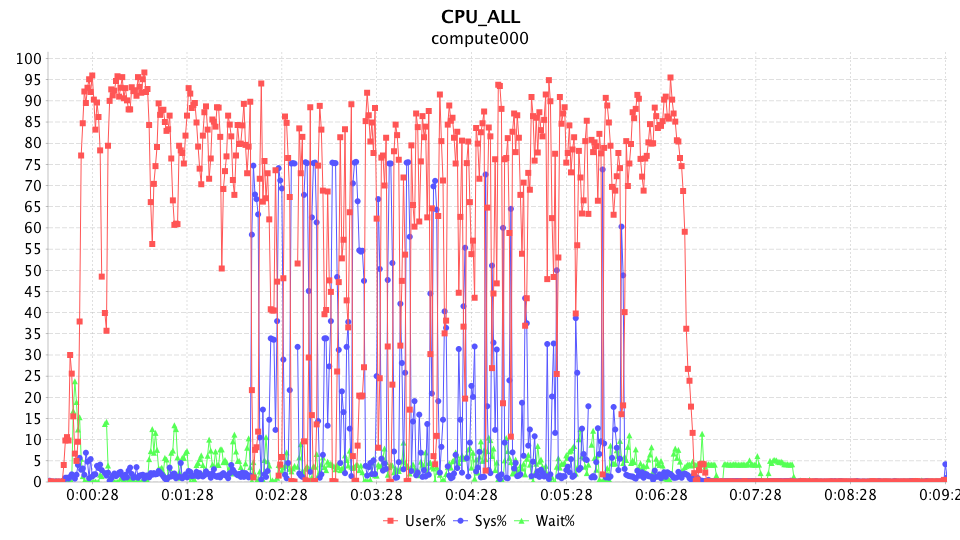
\includegraphics[width=1\linewidth]{figures/FFT131_576_CPU.png}
  \caption{CPU Usage}
  \label{FFT131_576_CPU}
\end{subfigure}
\begin{subfigure}{1\textwidth}
  \centering
  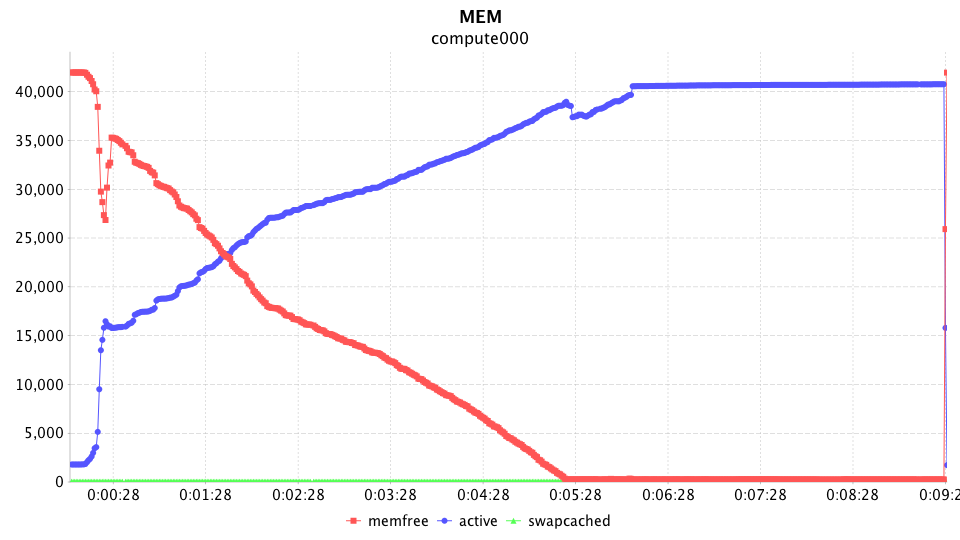
\includegraphics[width=1\linewidth]{figures/FFT131_576_MEM.png}
  \caption{Memory Usage}
  \label{FFT131_576_MEM}
\end{subfigure}
\caption{Resource Usage of FFT with Subvolume size 3x3x3 and 576 Cores}
\label{FFT131_576}
\end{figure}


\begin{figure}[h]
\centering
\begin{subfigure}{1\textwidth}
  \centering
  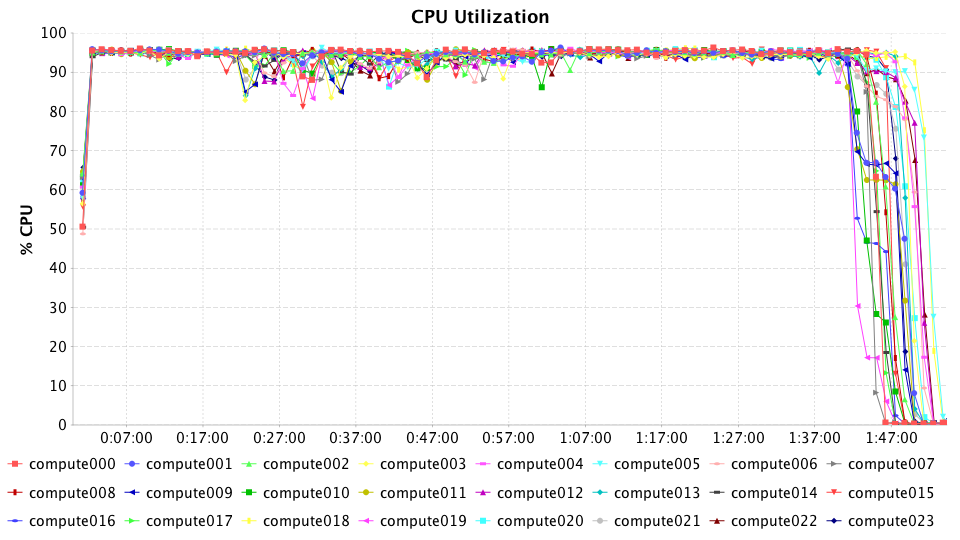
\includegraphics[width=1\linewidth]{figures/FFT474_576_CPU.png}
  \caption{CPU Usage}
  \label{FFT474_576_CPU}
\end{subfigure}
\begin{subfigure}{1\textwidth}
  \centering
  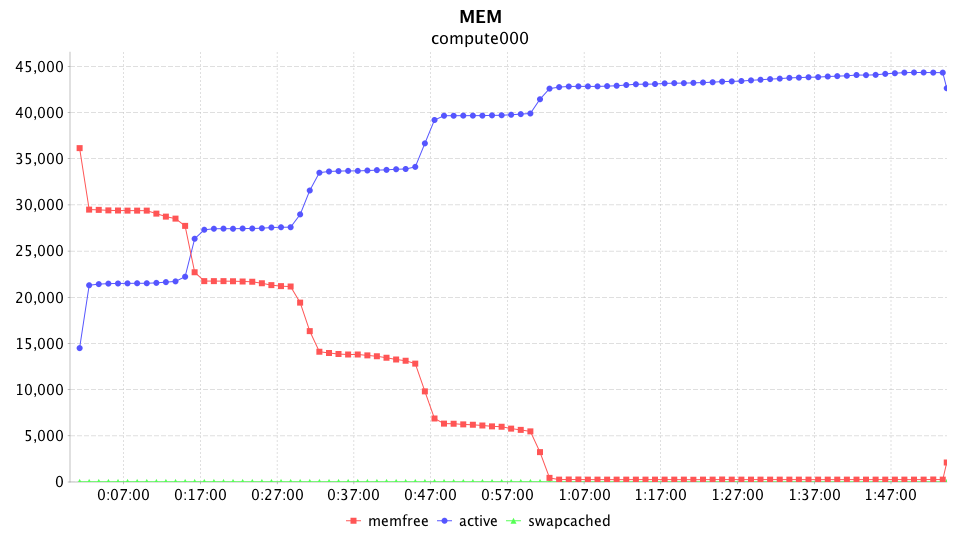
\includegraphics[width=1\linewidth]{figures/FFT474_576_MEM.png}
  \caption{Memory Usage}
  \label{FFT474_576_MEM}
\end{subfigure}
\caption{Resource Usage of FFT with Subvolume size 9x9x9 and 576 Cores}
\label{FFT474_576}
\end{figure}


\subsection{Performance Analysis of Histogram}

In Figure \ref{HistSpeedup}, the best result comes from 1 line per split running with 576 cores. In 1 line per split with different cores, the speed up factors increase with more cores added. The actual number of cores on whole workers is 288 (each node has 12 cores), and 576 cores are running in hyper-threading mode, so the performance only boost slightly from 288 cores to 576 cores. With increasing split size, the performance decreases drastically, which need deep analysis. 

Before diving into huge amount of metrics data, it is very important to know the struct of programm. While computing histogram, the first step is get minimum and miximum value of dataset, create bucket array basing on bucket count from input paramater, and then iterate whole dataset and put every element to it's corresponding position in bucket array. Figure \ref{Hist1_576_CPU} shows the CPU usage of histogram configured with 1 line per split and 576 cores. It is clear that there are two stages: the first ridge gets minimum and maximum values, and the second one iterate all data and accumulate results. The CPU utilization quickly ramps to 90% and stay at same level until stage finish, so there is no much bottle neck and the performance is best among all configuration.

But in Figure \ref{Hist10_72} and \ref{Hist10_288}, there are several fluctuations in utilization of CPU. The split size increases from 1 line to 10 lines, but the executation time of stage 1 has slowed down almost 6 times. By digging into the implementation codes of Spark as shown in List \ref{SparkCodeHist}, we ascribe it to the foldRight function. 

\lstset{language=Java,frame=single}
\begin{lstlisting}[float,caption= Codes Snippet of Histogram in Spark , label=SparkCodeHist]
    // Compute the minimum and the maximum
    val (max: Double, min: Double) = self.mapPartitions {items=>
      Iterator(items.foldRight(Double.NegativeInfinity,
        Double.PositiveInfinity)((e:Double,x:Pair[Double,Double])=>
        (x._1.max(e), x._2.min(e))))
    }.reduce {(maxmin1,maxmin2)=>
      (maxmin1._1.max(maxmin2._1),maxmin1._2.min(maxmin2._2))
    }
\end{lstlisting}


%%%%%%%%%%%%%%%%%%%%%%%%%%%%%%%%%%%%%%%%%%%%%%%%%%%%%%%
\begin{figure}[h]
%\centering
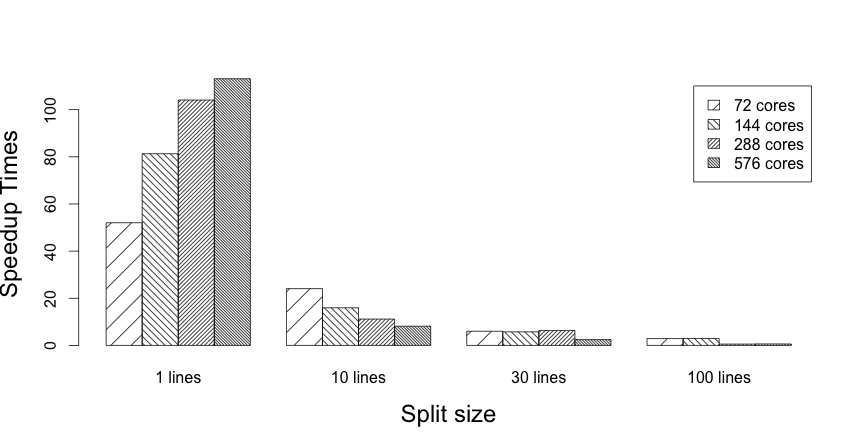
\includegraphics[scale=.50]{figures/HistSpeedup.png}
\caption{Speedup of Histogram Computation Codes}
\label{HistSpeedup}
\end{figure}
%%%%%%%%%%%%%%%%%%%%%%%%%%%%%%%%%%%%%%%%%%%%%%%%%%%%%%%

%%%%%%%%%%%%%%%%%%%%%%%%%%%%%%%%%%%%%%%%%%%%%%%%%%%%%%%
\begin{figure}[h]
%\centering
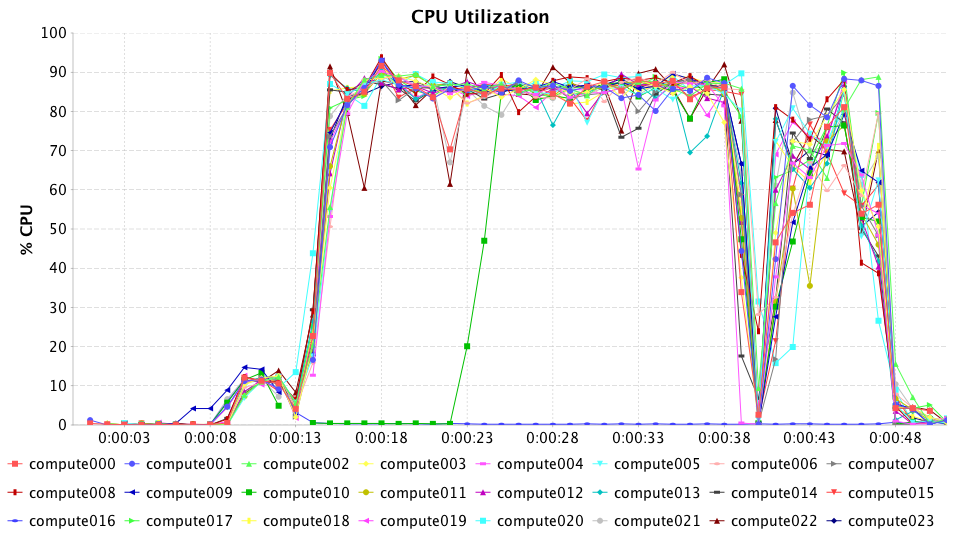
\includegraphics[scale=.50]{figures/Hist1_576_CPU.png}
\caption{CPU Usage of Histogram with 1 Line per Split and 576 Cores }
\label{Hist1_576_CPU}
\end{figure}
%%%%%%%%%%%%%%%%%%%%%%%%%%%%%%%%%%%%%%%%%%%%%%%%%%%%%%%

\ifx true false

\begin{figure}[h]
\centering
\begin{minipage}{.5\textwidth}
  \centering
  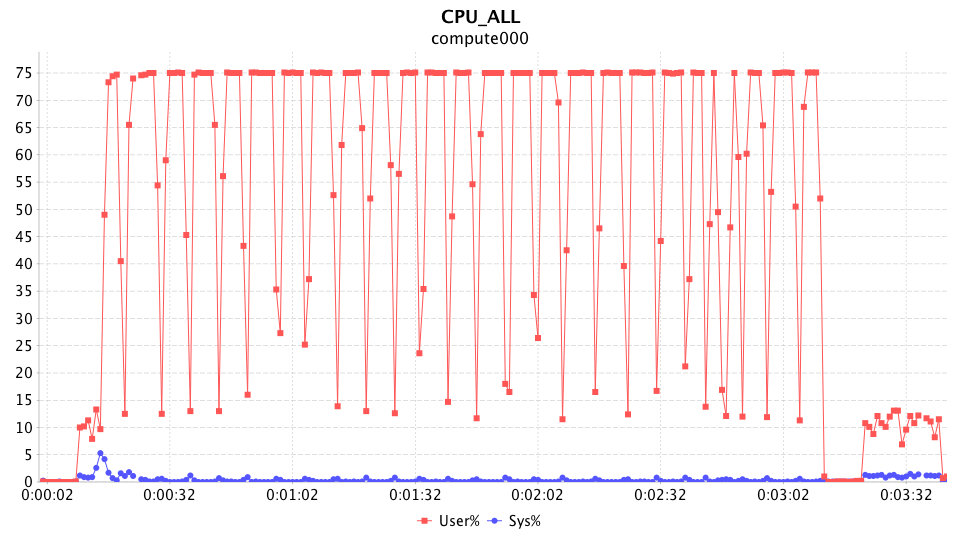
\includegraphics[width=.4\linewidth]{figures/Hist10_72_CPU.png}
  \caption{CPU Usage of Histogram with 10 Lines per Split and 72 Cores}
  \label{Hist10_72_CPU}
\end{minipage}%
\begin{minipage}{.5\textwidth}
  \centering
  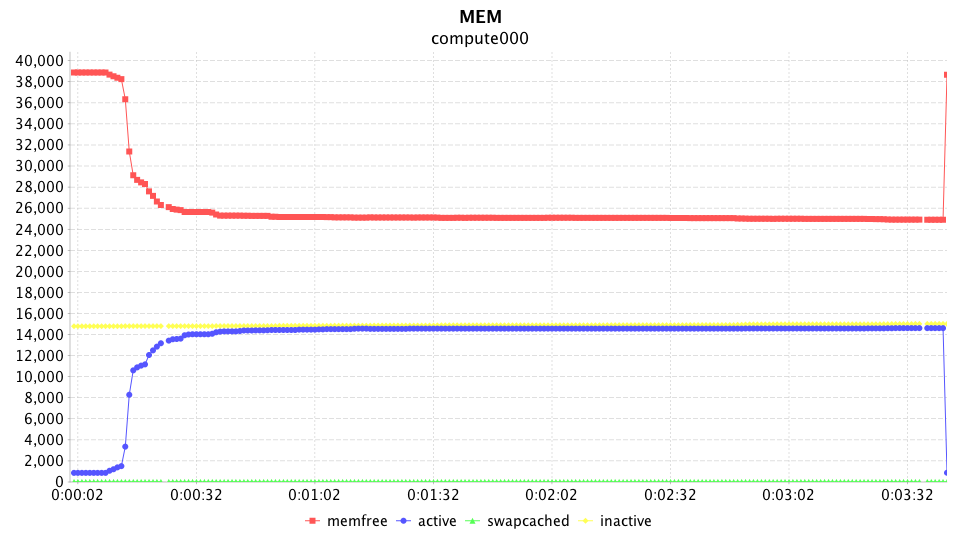
\includegraphics[width=.4\linewidth]{figures/Hist10_72_MEM.png}
  \caption{Memory Usage of Histogram with 10 Lines per Split and 72 Cores}
  \label{Hist10_72_MEM}
\end{minipage}
\end{figure}

\fi

\begin{figure}[h]
\centering
\begin{subfigure}{1\textwidth}
  \centering
  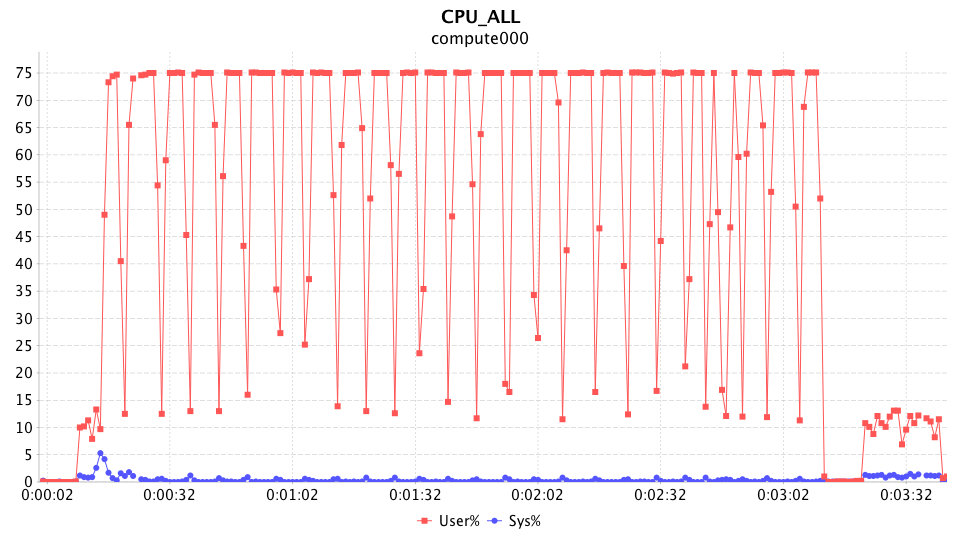
\includegraphics[width=1\linewidth]{figures/Hist10_72_CPU.png}
  \caption{CPU Usage}
  \label{Hist10_72_CPU}
\end{subfigure}
\begin{subfigure}{1\textwidth}
  \centering
  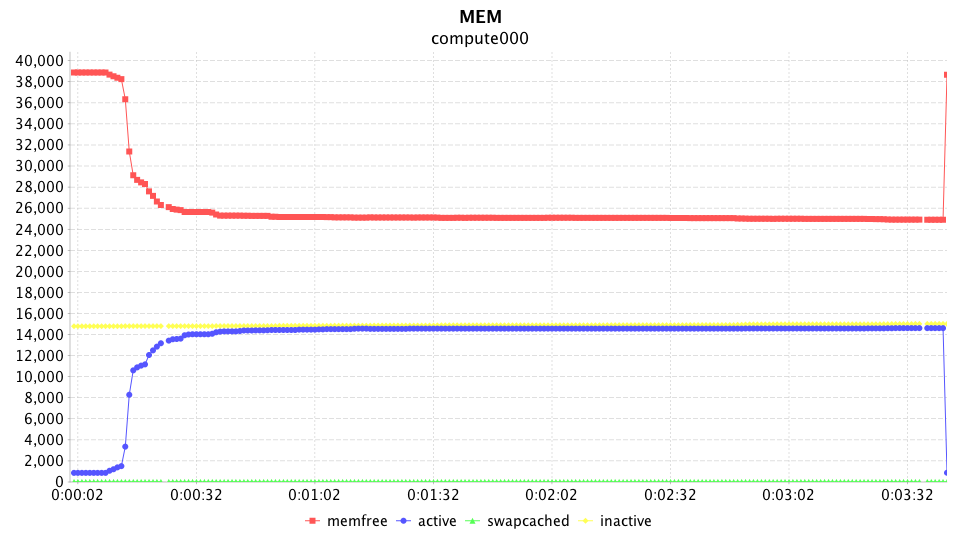
\includegraphics[width=1\linewidth]{figures/Hist10_72_MEM.png}
  \caption{Memory Usage}
  \label{Hist10_72_MEM}
\end{subfigure}
\caption{Resource Usage of Histogram with 10 Lines per Split and 72 Cores}
\label{Hist10_72}
\end{figure}

\begin{figure} [h]
\centering
\begin{subfigure}{1\textwidth}
  \centering
  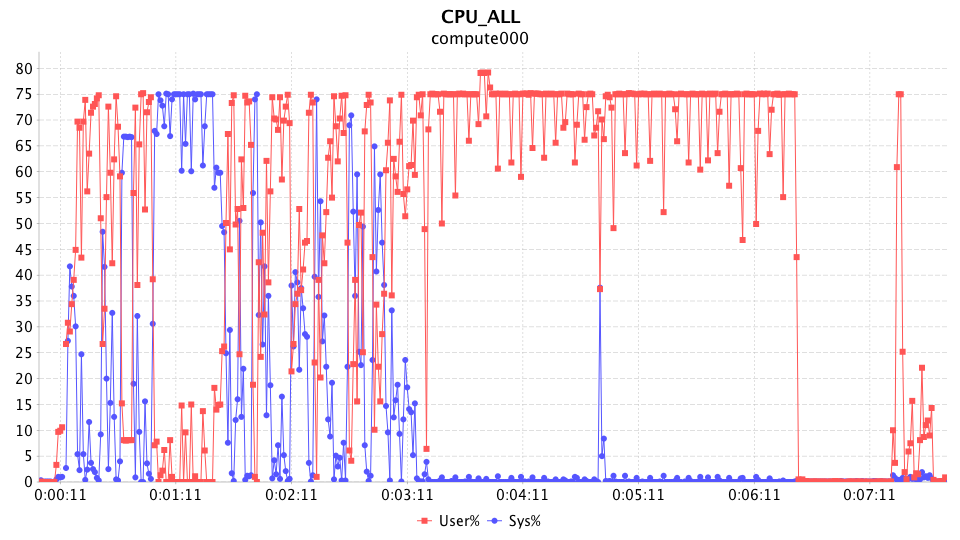
\includegraphics[width=1\linewidth]{figures/Hist10_288_CPU.png}
  \caption{CPU Usage}
  \label{Hist10_288_CPU}
\end{subfigure}
\begin{subfigure}{1\textwidth}
  \centering
  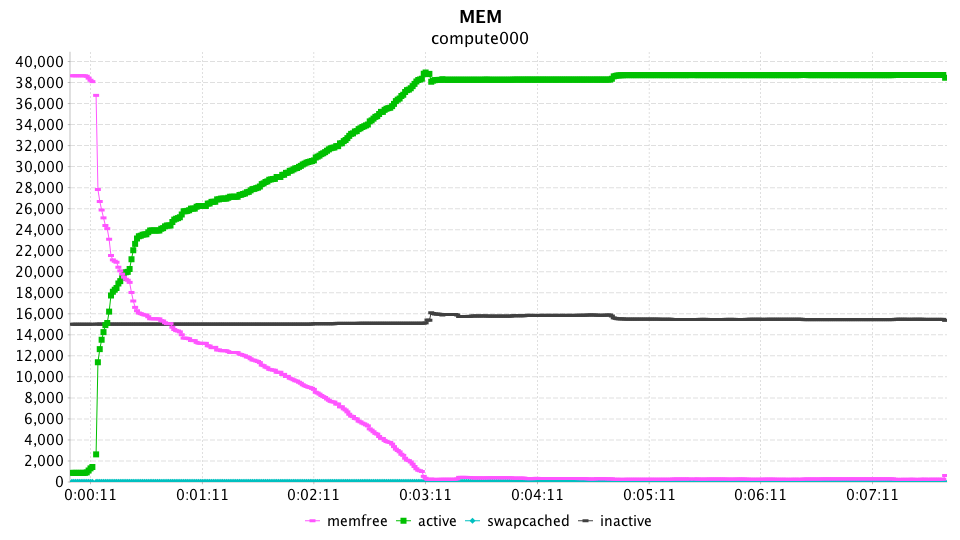
\includegraphics[width=1\linewidth]{figures/Hist10_288_MEM.png}
  \caption{Memory Usage}
  \label{Hist10_288_MEM}
\end{subfigure}
\caption{Resource Usage of Histogram with 10 Lines per Split and 288 Cores}
\label{Hist10_288}
\end{figure}

\subsection{Performance Analysis of Jacobi iteration}

%%%%%%%%%%%%%%%%%%%%%%%%%%%%%%%%%%%%%%%%%%%%%%%%%%%%%%%
\begin{figure}[h]
%\centering
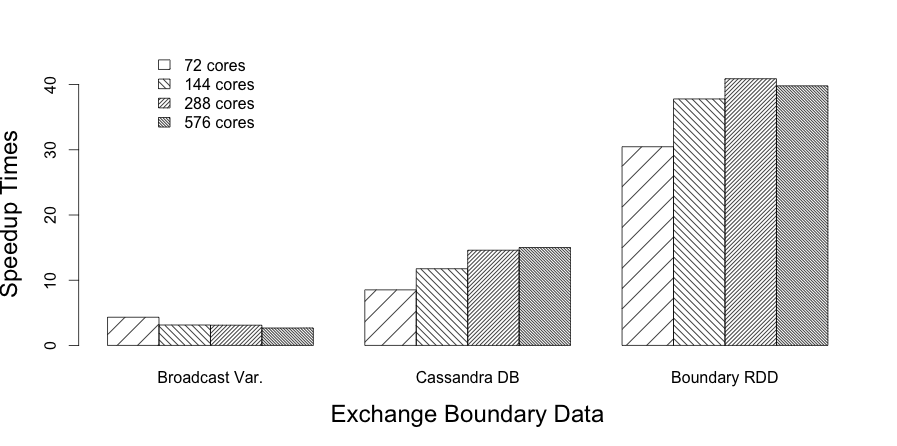
\includegraphics[scale=.50]{figures/JacobiSpeedup.png}
\caption{Speedup of Jacobi Stencil Codes}
\label{JacobiSpeedup}
\end{figure}
%%%%%%%%%%%%%%%%%%%%%%%%%%%%%%%%%%%%%%%%%%%%%%%%%%%%%%%


\begin{figure} [h]
\centering
\begin{subfigure}{1\textwidth}
  \centering
  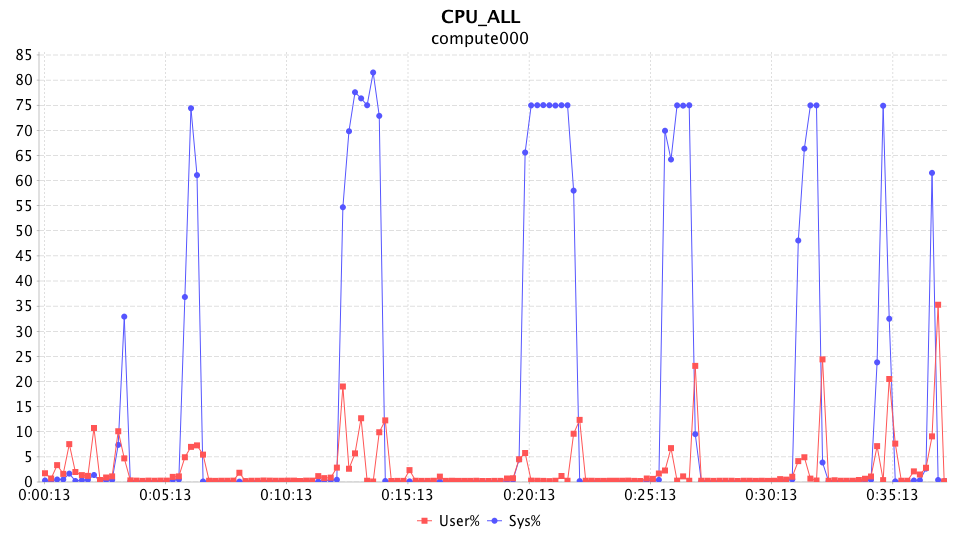
\includegraphics[width=1\linewidth]{figures/JacobiBC131_576_CPU.png}
  \caption{CPU Usage}
  \label{JacobiBC131_576_CPU}
\end{subfigure}
%\begin{subfigure}{1\textwidth}
%  \centering
%  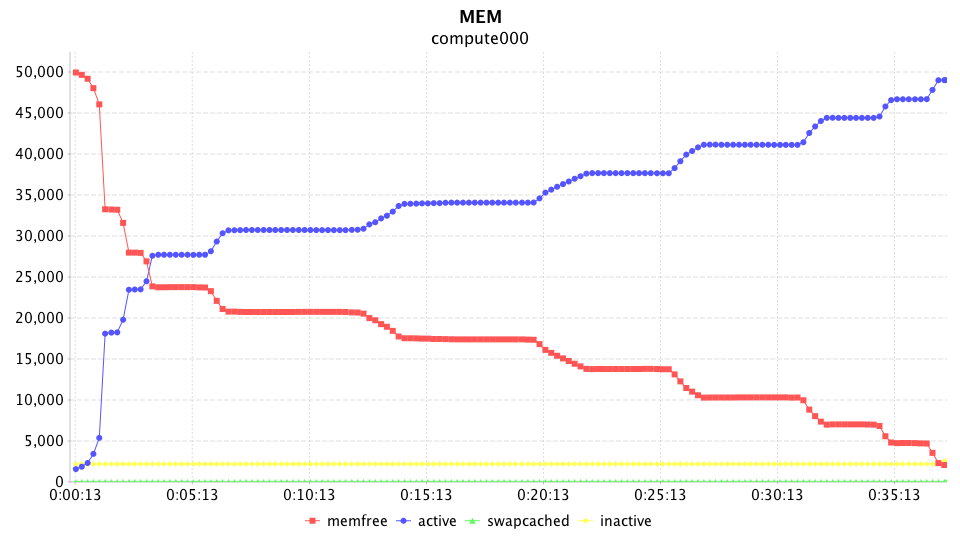
\includegraphics[width=1\linewidth]{figures/JacobiBC131_576_MEM.png}
%  \caption{Memory Usage}
%  \label{JacobiBC131_576_MEM}
%\end{subfigure}
\begin{subfigure}{1\textwidth}
  \centering
  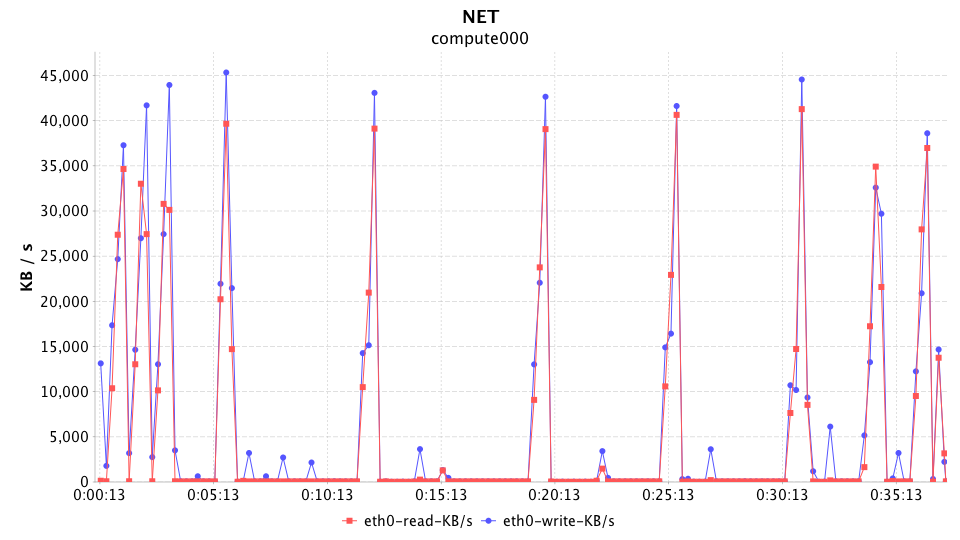
\includegraphics[width=1\linewidth]{figures/JacobiBC131_576_NET.png}
  \caption{Network Usage}
  \label{JacobiBC131_576_NET}
\end{subfigure}
\caption{Resource Usage of Jacobi Codes Using Broadcast Variables Sharing Data and Running with 576 Cores}
\label{JacobiBC131_576}
\end{figure}

\begin{figure} [h]
\centering
\begin{subfigure}{1\textwidth}
  \centering
  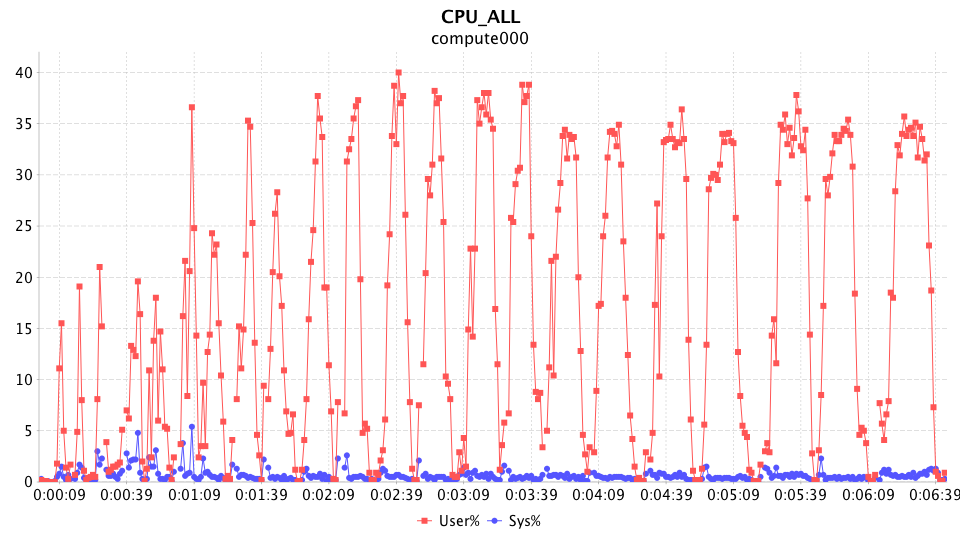
\includegraphics[width=1\linewidth]{figures/JacobiDB131_576_CPU.png}
  \caption{CPU Usage}
  \label{JacobiDB131_576_CPU}
\end{subfigure}
%\begin{subfigure}{1\textwidth}
%  \centering
%  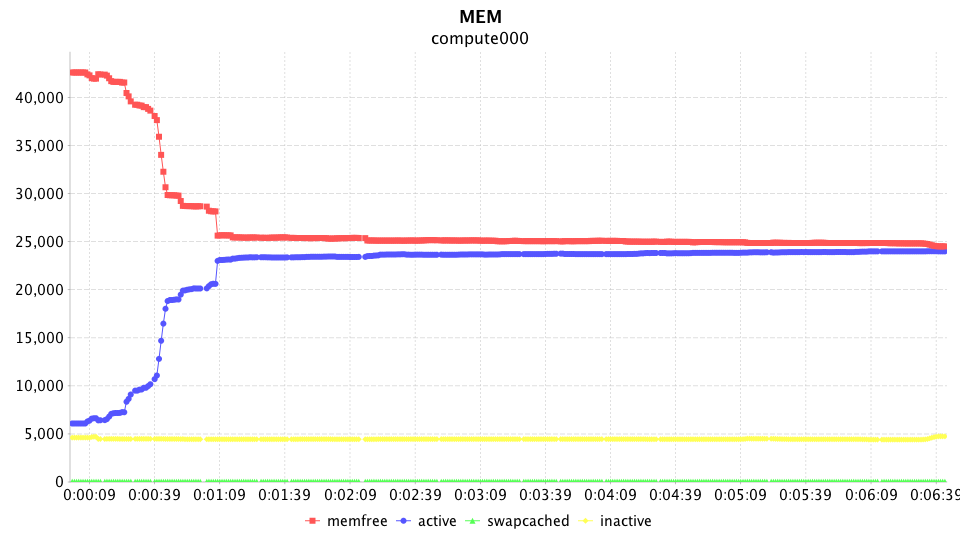
\includegraphics[width=1\linewidth]{figures/JacobiDB131_576_MEM.png}
%  \caption{Memory Usage}
%  \label{JacobiDB131_576_MEM}
%\end{subfigure}
\begin{subfigure}{1\textwidth}
  \centering
  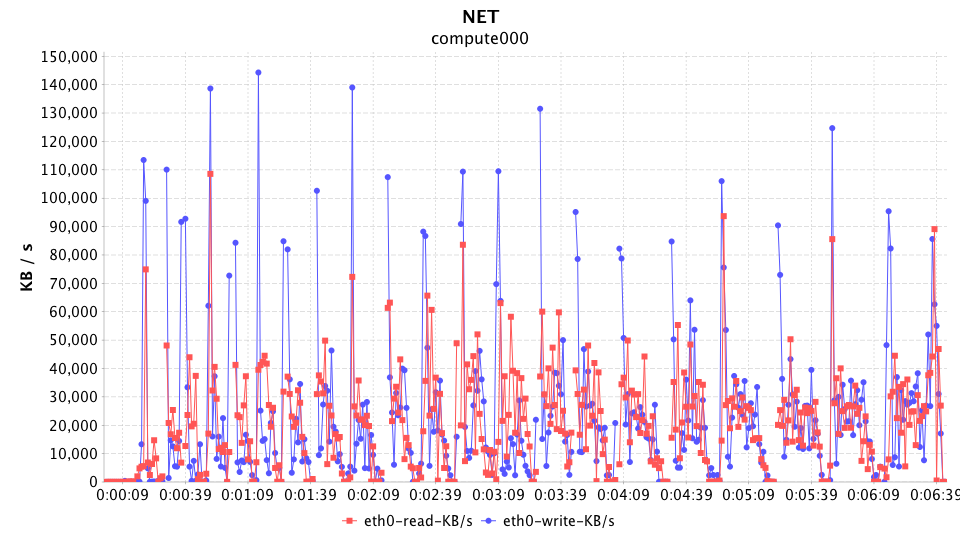
\includegraphics[width=1\linewidth]{figures/JacobiDB131_576_NET.png}
  \caption{Network Usage}
  \label{JacobiDB131_576_NET}
\end{subfigure}
\caption{Resource Usage of Jacobi Codes Using Cassandra DB Sharing Data and Running with 576 Cores}
\label{JacobiDB131_576}
\end{figure}

\begin{figure} [h]
\centering
\begin{subfigure}{1\textwidth}
  \centering
  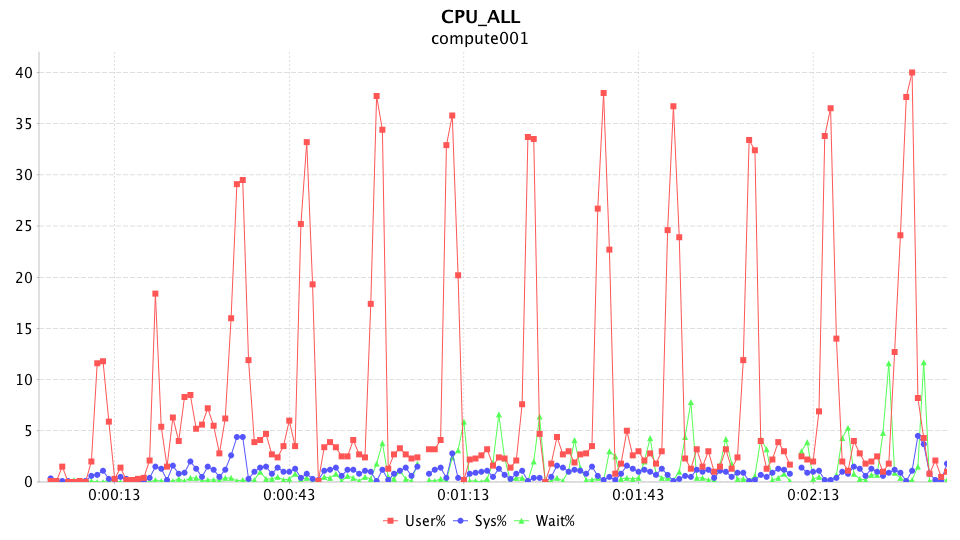
\includegraphics[width=1\linewidth]{figures/JacobiBRDD131_576_CPU.png}
  \caption{CPU Usage}
  \label{JacobiBRDD131_576_CPU}
\end{subfigure}
%\begin{subfigure}{1\textwidth}
%  \centering
%  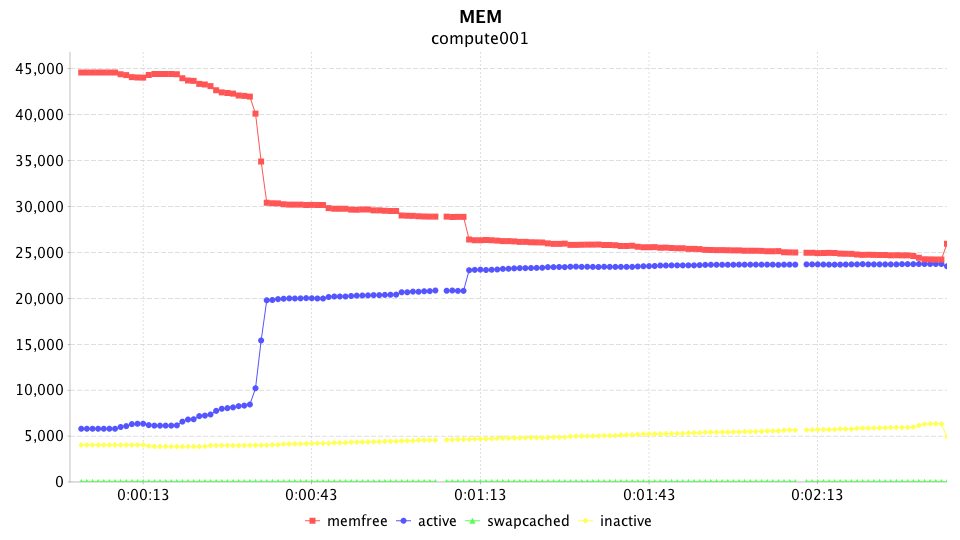
\includegraphics[width=1\linewidth]{figures/JacobiBRDD131_576_MEM.png}
%  \caption{Memory Usage}
%  \label{JacobiBRDD131_576_MEM}
%\end{subfigure}
\begin{subfigure}{1\textwidth}
  \centering
  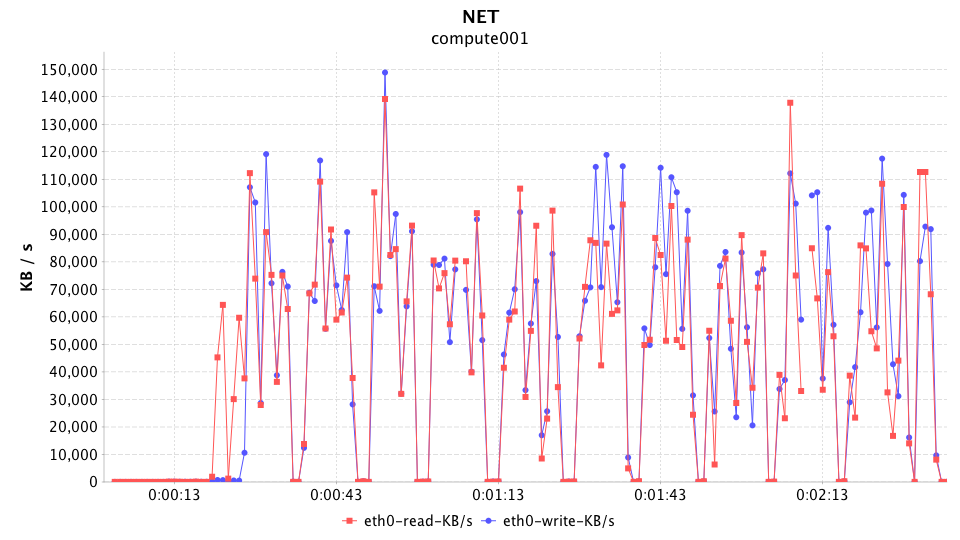
\includegraphics[width=1\linewidth]{figures/JacobiBRDD131_576_NET.png}
  \caption{Network Usage}
  \label{JacobiBRDD131_576_NET}
\end{subfigure}
\caption{Resource Usage of Jacobi Codes Using Boundary RDD Sharing Data and Running with 576 Cores}
\label{JacobiBRDD131_576}
\end{figure}




